
%% * Define trajectories
%% * Define returns
%% * Define policies
%% * Define State-value functions
%% * Define Action-value functions
%% * Present the types of solution methods

\subsection{The solution} \title{Defining the solutions} \author{} \date{}
\begin{frame}[plain,c]
    \titlepage
\end{frame}

\begin{frame}
    \frametitle{Policies $\pi$}
    \begin{itemize}
        \item Policies are mappings that from states $s_{t}$ that the agent
              might currently be in, to actions $a_{t}$ that the agent should
              take in those states.
              \begin{figure}
                \centering
                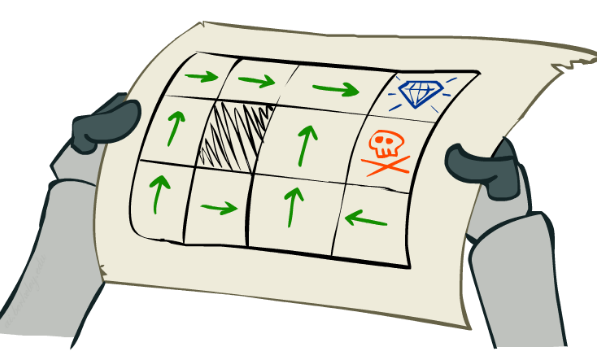
\includegraphics[width=0.5\textwidth]{./imgs/img_rl_policies.png}
              \end{figure}
        \pause
        \item These mappings could either be \textbf{Deterministic} (map a state
              to a single action) or \textbf{Stochastic} (map a state to a distribution
              over actions).
    \end{itemize}
\end{frame}

\begin{frame}
    \frametitle{Deterministic vs Stochastic Policies}
    \begin{figure}
        \centering
        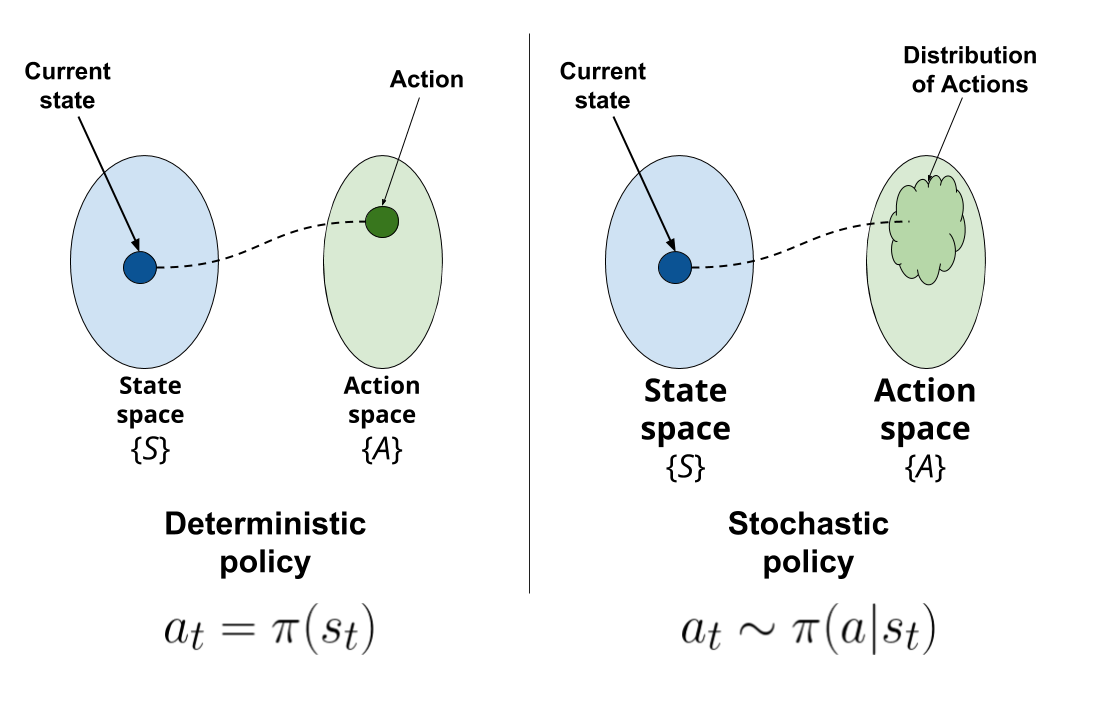
\includegraphics[width=0.9\textwidth]{./imgs/img_rl_policies_types.png}
    \end{figure}
\end{frame}

\begin{frame}
    \frametitle{Some more definitions}
    \begin{block}{Trajectories}
        A \textbf{trajectory} $\tau$ is a sequence of states-actions-rewards generated by running
        a policy in the environment.
        \begin{equation*}
            \tau = (s_{0},a_{0},r_{1},s_{1},a_{1},r_{2},\hdots)
        \end{equation*}
    \end{block}
    \pause
    \begin{block}{Returns}
        A \textbf{return} $G_{t}$ is the cummulative reward obtained from a given timestep
        onwards.
        \begin{equation*}
            G_{t} = \sum_{t'=1}^{T} r_{t' + t}
        \end{equation*}
    \end{block}
\end{frame}

\begin{frame}
    \frametitle{Optimal policies}
    \begin{block}{RL-objective}
        We can define the RL-objective using the previous concepts as follows:
        \begin{equation*}
            \pi^{*} = \arg \max_{\pi} \mathbb{E}_{\pi} \left \{ G_{t} \right \}
        \end{equation*}
        Where the policy $\pi^{*}$ is called the optimal policy.
    \end{block}
    \pause
    \begin{block}{Optimal Policy}
        An Optimal Policy $\pi^{*}$ is a policy (there could be many) that for any
        state $s \in S$, it gets more expected return than any other policy $\pi$
        at that same state $s$.
        \begin{equation*}
            \mathbb{E}_{\pi^{*}} \left \{ G_{t} | s_{t} = s \right \} \geq
            \mathbb{E}_{\pi} \left \{ G_{t} | s_{t} = s \right \}; \forall \pi, \forall s \in S
        \end{equation*}
    \end{block}
\end{frame}

\begin{frame}
    \frametitle{State-value functions}
    \begin{itemize}
        \item As explained earlier, the objective of the agent is to find the policy
              that for any state $s \in S$ it picks the action that maximizes expected
              return $\mathbb{E}_{\pi}\left \{ G_{t} | s_{t} = s \right \}$

        \pause

        \item Let's define the expected return starting at state $s_{t}=s$ and
              following policy $\pi$ as the \textbf{State-Value Function} $V_{\pi}(s)$.
              \begin{equation*}
                V_{\pi}(s) = \mathbb{E}_{\pi} \left \{ G_{t} | s_{t} = s \right \}
              \end{equation*}
    \end{itemize}
\end{frame}

\begin{frame}
    \frametitle{State-value functions}
    \begin{figure}
        \centering
        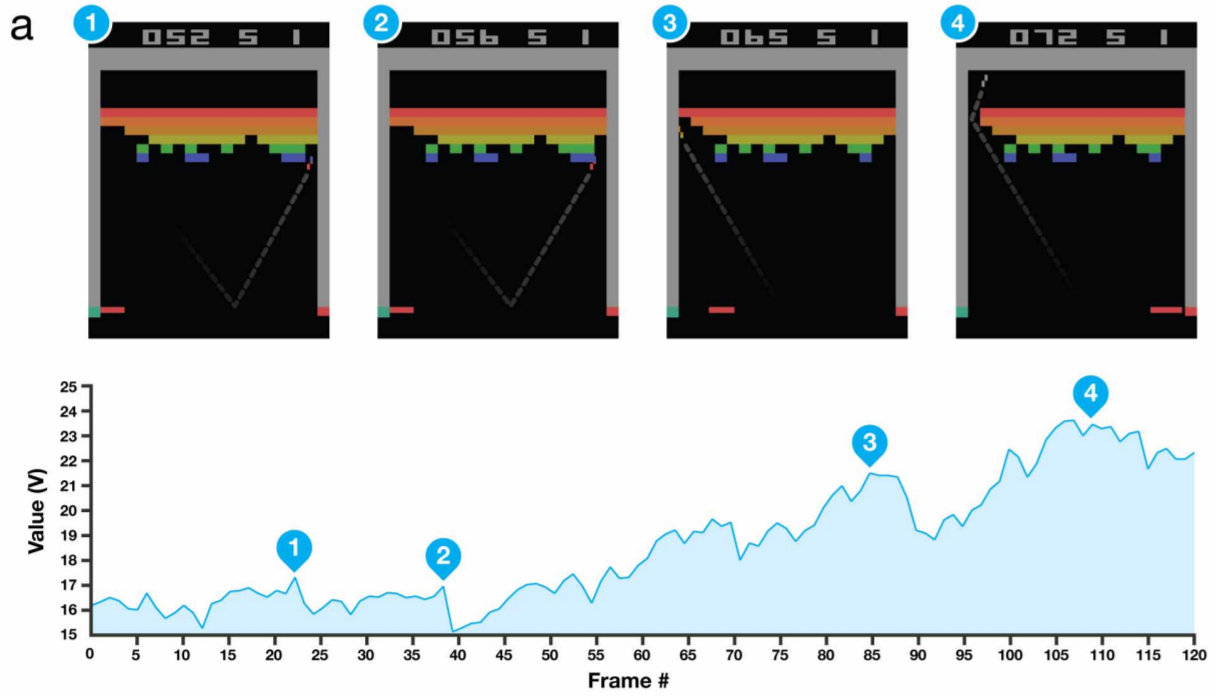
\includegraphics[width=0.9\textwidth]{./imgs/img_rl_vfunction_intuition.png}
    \end{figure}
\end{frame}

\begin{frame}
    \frametitle{Action-value functions}
    \begin{itemize}
        \item Similarly, we can define a function that tells us how well an action 
              $a_{t}=a$ would be if we take it in state $s_{t}=s$ and then follow
              the policy $\pi$ onwards.

        \pause

        \item We define this function as the \textbf{Action-Value Function} $Q_{\pi}(s,a)$
              \begin{equation*}
                Q_{\pi}(s,a) = \mathbb{E}_{\pi} \left \{ G_{t} | s_{t} = s, a_{t} = a \right \}
              \end{equation*}
    \end{itemize}
\end{frame}

\begin{frame}
    \frametitle{Action-value functions}
    \begin{figure}
        \centering
        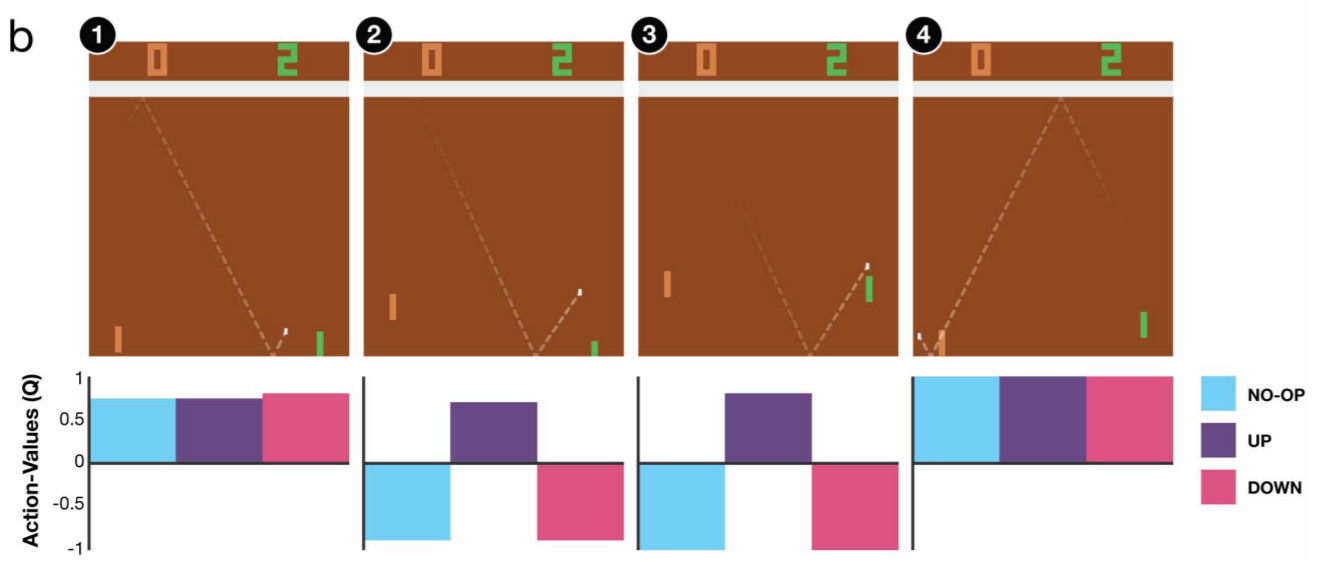
\includegraphics[width=0.9\textwidth]{./imgs/img_rl_qfunction_intuition.png}
    \end{figure}
\end{frame}